\chapter{Implementation and Results}
\label{chap:ImplementationAndResults}

The previous chapter detailed the architectural design and core methodologies for the \texttt{Arralac} compiler. This chapter transitions from design to practice, describing the concrete Haskell implementation that realizes this architecture.

First, I will examine the implementation of the core data structures, particularly the Trees That Grow (TTG) Abstract Syntax Tree (AST). Next, I will detail the type inference pipeline, focusing on the separation between constraint generation and solving. Finally, I will present concrete results, including the output for both successful and unsuccessful typechecking scenarios, and a demonstration of the functional Language Server Protocol (LSP) features.

\section{AST Implementation with Trees That Grow}
\label{sec:Implementation:AST}

As outlined in the design (\cref{sec:Design:AST}), the AST is built using the Trees That Grow (TTG) pattern to ensure extensibility and to facilitate annotations. The core data types, \texttt{SynTerm} for expressions, \texttt{SynType} for syntactic types, and \texttt{Type} for non-syntactic types are parameterized by a type variable \texttt{x} that represents the current compiler pass (e.g., \texttt{CompRn} for Renamed, \texttt{CompTc} for Typechecked, \texttt{CompZn} for Zonked).

Unlike a simpler AST where fields have concrete types, every component of an \texttt{Arralac} AST node is defined by a type family. This allows the structure of a node to be radically different across passes. The generic definition for \texttt{SynTerm} is shown below.

\begin{minted}[frame=lines,label={The Generic \texttt{SynTerm} Data Type in \texttt{Language.Arralac.Syntax.TTG.SynTerm}}]{haskell}
data SynTerm x
  = -- | \ (x :: a) -> x
    SynTerm'ALam (XSynTerm'ALam' x) (XSynTerm'ALam'Var x) 
                 (XSynTerm'ALam'Type x) (XSynTerm'ALam'Body x)
  | -- | (f x) :: Int
    SynTerm'Ann (XSynTerm'Ann' x) (XSynTerm'Ann'Term x) 
                (XSynTerm'Ann'Type x)
  -- ... other constructors
\end{minted}

The power of TTG is realized through the instantiation of these type families for each specific compiler pass. For the typechecking pass (\texttt{CompTc}), the extension point fields (e.g., \texttt{XSynTerm'Ann'}) are instantiated with a \texttt{TcAnno} record. This record is crucial for tooling, as it contains the inferred type for that node, which is later used by the language server.

\begin{minted}[frame=lines,label={Type Family Instantiation for the Typechecked Pass}]{haskell}
-- In Language.Arralac.Syntax.Local.SynTerm.Tc
type instance XSynTerm'Ann'Term CompTc = SynTerm CompTc
type instance XSynTerm'Ann'Type CompTc = SynType CompTc

-- In Language.Arralac.Syntax.Local.Extension.Tc
-- The AST node is annotated with its type after typechecking.
type instance XSynTerm'Ann' CompTc = TcAnno
data TcAnno = TcAnno { annoSrcLoc :: SrcSpan, annoType :: Expected TcType }
\end{minted}

This approach provides a compile-time, type-safe guarantee that pass-specific information is only available in the AST after that pass has successfully completed.

\section{The Type Inference and Solving Pipeline}
\label{sec:Implementation:Pipeline}

The implementation of the type inference engine closely follows the constraint-based design laid out in \cref{sec:Design:TypeInference}. The process is divided into distinct, sequential stages, each managed by its own set of modules.

\subsection{Constraint Generation (\texttt{Typechecker})}
The first phase, implemented primarily in the \texttt{Language.Arralac.Typechecker.TcTerm} module, traverses the renamed AST to produce a set of wanted constraints. The \texttt{unify} function merely emits canonical equality constraints with a metavariable on the left-hand side and a monotype on the right-hand side.

\begin{itemize}
  \item \textbf{Bidirectional Logic:} The core function, \texttt{tcRho}, implements the bidirectional algorithm. When called in inference mode (via the \texttt{inferRho} wrapper), it is passed a new mutable reference (\texttt{Expected (IORef TcType)}) to hold the resulting type. When called in checking mode (via \texttt{checkRho}), it consumes the expected type passed to it.

  \item \textbf{Implication Constraints:} At each point where skolemization is required --- specifically, within the \texttt{checkSigma} function when checking an expression against a polymorphic type --- the typechecker enters a deeper scope. This is implemented by the helper function \texttt{pushLevelAndCaptureConstraints}. This function increments the current \texttt{TcLevel}, captures all new constraints generated within its scope, and packages them into an \texttt{Implic} constraint, which bundles the new skolem variables created at the current level with the constraints at a deeper level in which these skolems may occur. This directly models the scoped nature of polymorphism.
\end{itemize}

\subsection{Constraint Solving (\texttt{Solver})}
The set of \texttt{WantedConstraints} generated by the typechecker is passed to the solver, implemented in \texttt{Language.Arralac.Solver.Solve}. The solver iteratively processes a worklist of simple equality constraints (\texttt{wc\_simple}).

\begin{itemize}
  \item \textbf{Occurs and Level Checks:} Before attempting to unify a metavariable with a type, the solver performs two critical checks implemented in \texttt{Language.Arralac.Solver.Check}. First, an \textbf{occurs check} ensures the metavariable does not appear within the right-hand side of the type, preventing infinite types like $a ~ a \rightarrow a$. Second, a \textbf{level check} verifies that the type on the right-hand side does not contain any skolem variables with a level deeper than the metavariable. This check is the concrete implementation of the skolem escape rule discussed in the design chapter.

  \item \textbf{Unification:} If the checks pass, the solver unifies the variable by writing to the metavariable's mutable \texttt{IORef}. Constraints within implications are solved recursively within their own, deeper-level scope. Any constraints that cannot be solved (e.g., due to a type mismatch or a failed check) trigger an exception. When a metavariable contains a type, the \texttt{unify} function (defined in \texttt{Solver.Unify}) tries to generate new constraints by equating the contained type and the type on the right-hand side of the constraint. Therefore, the solver may need several iterations to solve constraints.
\end{itemize}

\subsection{Finalization (\texttt{Zonker})}
After the solver has completed, the \texttt{Zonker}, implemented in \texttt{Language.Arralac.Zonker.Zn.Zonk}, traverses the now-typed AST. It recursively resolves the \texttt{IORef} of each metavariable, replacing it with its final, unified fully zonked type. Metavariables that were not solved are explicitly renamed to indicate their status (e.g., \texttt{a\_Unsolved\_11}), producing a final AST that is free of mutable references and ready for code generation or evaluation.

\section{Results and System in Action}
\label{sec:Implementation:Results}

This section demonstrates the functionality of the implemented system using both positive and negative test cases, validating the core mechanisms of the type system.

\subsection{A Positive Case: Higher-Rank Polymorphism}
To test the correct handling of higher-rank types, I use a program that requires passing a polymorphic function as an argument. The following program, \texttt{Program1.arralac}, defines a function \texttt{applyMyShow} that expects a polymorphic function of type \texttt{forall b. b -> String}.

\begin{minted}[frame=lines,label={Program1.arralac}]{haskell}
let
  applyMyShow =
    (\x. \y. x y)
      :: forall a. (forall b. b -> String) -> a -> String
in
let
  myShow = \x. "Hello"
in
applyMyShow myShow
\end{minted}

Running the \texttt{Arralac} CLI to typecheck the program produces a fully-annotated AST. The output in \Cref{fig:typecheck-output} shows that the system correctly inferred and propagated the types. Crucially, the lambda-bound variable \texttt{x\_1} is correctly assigned its higher-rank type from the annotation, and the final type correctly reflects that the type variable \texttt{a} was unconstrained and thus remains unsolved.

\begin{figure}[h]
  \centering
  \begin{minted}[frame=lines,fontsize=\small]{console}
$ nix run .#arralac -- typecheck arralac/test/data/Program1.arralac

(let
  -- Correct higher-rank type for applyMyShow
  applyMyShow_0 = 
    (\(x_1 :: forall b_4. b_4 -> String).
       (\(y_2 :: a_9). (x_1 :: a_9 -> String) (y_2 :: a_9) :: String
       ) :: a_9 -> String
    ) :: (forall b_4. b_4 -> String) -> a_Unsolved_11 -> String
in
  (let myShow_7 = (\(x_8 :: b_13). "Hello") :: b_13 -> String
   in (applyMyShow_0 (myShow_7)) :: a_Unsolved_11 -> String
  ) :: a_Unsolved_11 -> String
) :: a_Unsolved_11 -> String
\end{minted}
  \caption{Typechecking output for \texttt{Program1.arralac} (compacted).}
  \label{fig:typecheck-output}
\end{figure}

The evaluator correctly reduces the program to its weak head normal form (WHNF), as shown in \Cref{fig:evaluate-output}.

\begin{figure}[h]
  \centering
  \begin{minted}[frame=lines]{console}
$ nix run .#arralac -- evaluate whnf arralac/test/data/Program1.arralac

\y_2. (\x_8. "Hello") (y_2)
\end{minted}
  \caption{Evaluation output for \texttt{Program1.arralac}.}
  \label{fig:evaluate-output}
\end{figure}

\subsection{A Negative Case: Skolem Escape Detection}
To validate the robustness of the solver, a negative test case was created to trigger a skolem escape. The following program attempts to unify an outer-scope metavariable with an inner-scope skolem, which should be rejected.

\begin{minted}[frame=lines,label={SkolemEscape.arralac}]{haskell}
let 
  myRun = \(x :: forall a b. a -> b). 
    (let myBad = \y. y x in myBad)
in
  myRun
\end{minted}

When run through the typechecker and solver, the solver correctly identifies the illegal unification and reports a level check failure, as shown in \Cref{fig:skolem-escape-error}. This directly validates that the level-based checking mechanism is working as designed.

\begin{figure}[h]
  \centering
  \begin{minted}[frame=lines,fontsize=\small]{console}
$ nix run .#arralac -- typecheck arralac/test/data/Program2.arralac
CallStack (from HasCallStack):
  SolverErrorWithCallStack, called at src/Language/Arralac/Solver/Error.hs:25:24
  dieSolver, called at src/Language/Arralac/Solver/Check.hs:51:5
Skolem escape!
The variable:
  a_7[ID 7, L 0, Meta, Unknown span: No location]
has the TcLevel:
  L 0
but the type variable:
  a_11[ID 11, L 1, Meta, Unknown span: No location]
has a larger TcLevel:
  L 1
in the constraint:
...
\end{minted}
  \caption{Error message demonstrating successful skolem escape detection.}
  \label{fig:skolem-escape-error}
\end{figure}

\subsection{Interactive Tooling: The Language Server}
The implementation includes a functional language server that leverages the annotated AST to provide on-the-fly diagnostics and type information. \Cref{fig:lsp-demo} demonstrates two key features in Visual Studio Code: (1) hovering over an identifier (\texttt{applyMyShow}) to see its inferred polymorphic type, and (2) an error diagnostic for an unbound variable (\texttt{myShowww}). This closes the loop between the compiler's internal representations and a useful, interactive user experience.

\begin{figure}[h!]
  \centering
  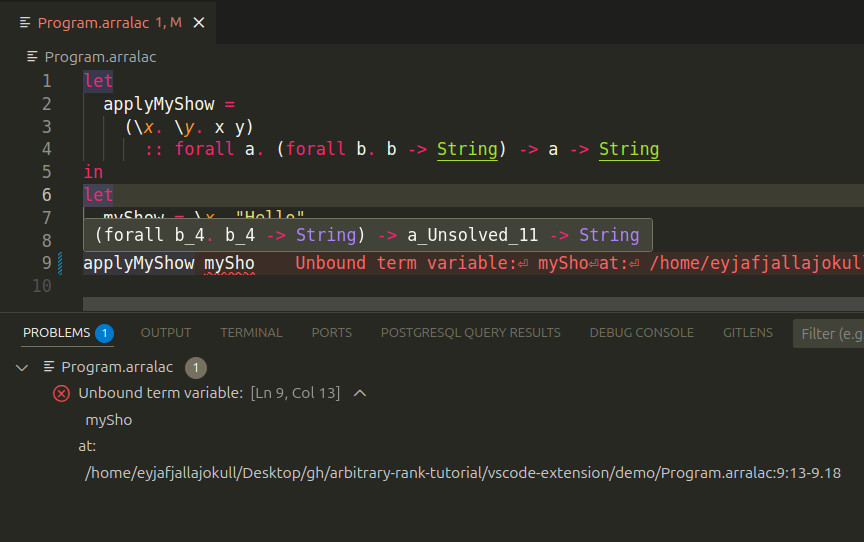
\includegraphics[width=0.9\textwidth]{VSCode.png}
  \caption{LSP features: type on hover and error diagnostics.}
  \label{fig:lsp-demo}
\end{figure}

\subsection{Codebase Characteristics}
The system was evaluated against several quality characteristics from the ISO 25010 standard.
\begin{itemize}
  \item \textbf{Modularity:} The codebase is highly modular, comprising 86 distinct Haskell modules, as shown by the \texttt{cloc} \footnote{The tool is available at \url{https://github.com/AlDanial/cloc}} analysis in \Cref{table:cloc}. This separation of concerns was critical for managing the complexity of the type inference engine.
  \item \textbf{Analysability:} The error-handling mechanism is designed for clear diagnostics. Each pipeline stage (e.g., Renamer, Typechecker, Solver) throws its own distinct error type, which captures a full call stack. This ensures that failures are easy to trace back to their source.
  \item \textbf{Installability:} The entire project is packaged with Nix, enabling a reproducible, single-line installation via the command \texttt{nix profile install}.
\end{itemize}

\begin{table}[h!]
  \centering
  \footnotesize
  \caption{Code Metrics for the \texttt{Arralac} Implementation Generated by \texttt{cloc}}
  \begin{tabular}{lrrrr}
    \toprule
    \textbf{Language} & \textbf{Files} & \textbf{Blank Lines} & \textbf{Comment Lines} & \textbf{Code Lines} \\
    \midrule
    Haskell           & 86             & 705                  & 1085                   & 3907                \\
    \midrule
    \textbf{SUM}      & \textbf{86}    & \textbf{705}         & \textbf{1085}          & \textbf{3907}       \\
    \bottomrule
  \end{tabular}
  \label{table:cloc}
\end{table}

This chapter has demonstrated that the design laid out previously has been successfully realized in a functional, well-structured, and non-trivial implementation. The system correctly handles higher-rank types, robustly rejects invalid programs, and provides modern tooling, fulfilling the primary objectives of this thesis.